\section{三角函数:A Picture for Karl's Students}
\subsection{环境:坐标轴}
启用 tikz 环境:
\begin{lstlisting}[style = latex]
    \begin{tikzpicture}
        ......
    \end{tikzpicture}
    \end{lstlisting}
画坐标轴:\\

\begin{figure}[H]
    \centering
    \begin{minipage}{0.35\linewidth}
        \centering
        \begin{tikzpicture}
            \draw (-1,0) -- (1,0);
            \draw (0,-1) -- (0,1);
            \end{tikzpicture}.
    \end{minipage}
    \begin{minipage}{0.55\linewidth}
        \begin{lstlisting}[style = latex-side]
    \begin{tikzpicture}
        \draw (-1,0) -- (1,0);
        \draw (0,-1) -- (0,1);
        \end{tikzpicture}.
        \end{lstlisting}
    \end{minipage}
    \caption{直线}
\end{figure}

两种 TikZ 画法:
\begin{enumerate}
    \item 通过 TikZ 环境,如上所述 
    \item 行内 TikZ ,如 \tikz \draw (-1,0) -- (1,0); 
\end{enumerate}

在不同的环境下 TikZ 有多种写法,这里不做说明 \\
\subsection{基本曲线}
\subsubsection{直线}
直线通过 \lstinline|\draw| 指令绘制:
\begin{lstlisting}[style = latex]
    \draw (x,y) -- (x,y) -- (x,y) ... ;
\end{lstlisting}
\begin{figure}[H]
    \centering
    \begin{minipage}{0.35\linewidth}
        \centering
        \tikz \draw (-1,0) -- (1,0) -- (0,1) -- (0,-1); 
    \end{minipage}
    \begin{minipage}{0.55\linewidth}
        \begin{lstlisting}[style = latex-side]
    \tikz \draw (-1,0) -- (1,0) -- (0,1) -- (0,-1); 
        \end{lstlisting}
    \end{minipage}
    \caption{直线}
\end{figure}

\subsubsection{曲线}
TikZ 的曲线原理在官方文档中没有详细解释,类似于贝塞尔曲线,我的理解如下:
\begin{itemize}
    \item 和直线类似,曲线也由点组成,和分为起止点,过程点
    \item 起止点为曲线的起点和终点,必须经过
    \item 过程点比必须经过,曲线有趋近的趋势
\end{itemize}

通过 \lstinline|\.. controls| 关键字控制曲线
\begin{lstlisting}[style = latex]
    Official: <start point> .. controls <1st control point> and <2nd control point> .. <end point>;
    Simple: \draw (x,y) .. controls (x,y) and (x,y) .. (x,y);
\end{lstlisting}
可以取消 .. 这样会让第一个点使用两次
\begin{figure}[H]
    \centering
    \begin{minipage}{0.35\linewidth}
        \centering
        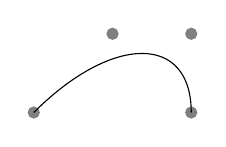
\begin{tikzpicture}
            \filldraw [gray] (0,0) circle [radius=2pt]
                            (1,1) circle [radius=2pt]
                            (2,1) circle [radius=2pt]
                            (2,0) circle [radius=2pt];
            \draw (0,0) .. controls (1,1) and (2,1) .. (2,0);
        \end{tikzpicture}
    \end{minipage}
    \begin{minipage}{0.55\linewidth}
        \begin{lstlisting}[style = latex-side]
    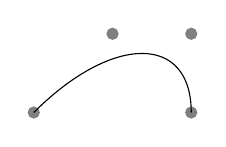
\begin{tikzpicture}
        \filldraw [gray] (0,0) circle [radius=2pt]
                         (1,1) circle [radius=2pt]
                         (2,1) circle [radius=2pt]
                         (2,0) circle [radius=2pt];
        \draw (0,0) .. controls (1,1) and (2,1) .. (2,0);
    \end{tikzpicture}
        \end{lstlisting}
    \end{minipage}
    \caption{曲线}
\end{figure}
继续坐标系的例子,可以画出伪半圆,注意下面的例子中,(0,1) 点既作为终点又作为起点
\begin{figure}[H]
    \centering
    \begin{minipage}{0.35\linewidth}
        \centering
        \begin{tikzpicture}
            \draw (-1.5,0) -- (1.5,0);
            \draw (0,-1.5) -- (0,1.5);
            \draw (-1,0) .. controls (-1,0.555) and (-0.555,1) .. (0,1)
            .. controls (0.555,1) and (1,0.555) .. (1,0);
        \end{tikzpicture}
    \end{minipage}
    \begin{minipage}{0.55\linewidth}
        \begin{lstlisting}[style = latex-side]
    \begin{tikzpicture}
        \draw (-1.5,0) -- (1.5,0);
        \draw (0,-1.5) -- (0,1.5);
        \draw (-1,0) .. controls (-1,0.555) and (-0.555,1) .. (0,1)
        .. controls (0.555,1) and (1,0.555) .. (1,0);
    \end{tikzpicture}
        \end{lstlisting}
    \end{minipage}
    \caption{带半圆曲线的坐标轴}
\end{figure}

\subsubsection{椭圆}
可以通过如下方式绘制椭圆
\begin{lstlisting}[style = latex]
    \draw <point> <category> [args];
\end{lstlisting}
其中:<point>:圆心 <category>:椭圆类型 [args]:对应的参数
例如下面绘制的圆和椭圆

\begin{figure}[H]
    \centering
    \begin{minipage}{0.12\textwidth}
        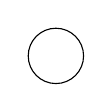
\begin{tikzpicture}
            \draw (0,0) circle [radius=10pt];
        \end{tikzpicture}
    \end{minipage}
    \begin{minipage}{0.12\textwidth}
        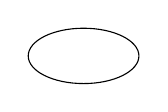
\begin{tikzpicture}
            \draw (0,0) ellipse [x radius=20pt, y radius=10pt];
        \end{tikzpicture}
    \end{minipage}
    \begin{minipage}{0.55\textwidth}
        \begin{lstlisting}[style = latex-side]
    \draw (0,0) circle [radius=10pt];
    \draw (0,0) ellipse [x radius=20pt, y radius=10pt];
        \end{lstlisting}
    \end{minipage}
    \caption{椭圆}
\end{figure}

继续在坐标轴上加上圆

\begin{figure}[H]
    \centering
    \begin{minipage}{0.35\linewidth}
        \centering
        \begin{tikzpicture}
            \draw (-1.5,0) -- (1.5,0);
            \draw (0,-1.5) -- (0,1.5);
            \draw (0,0) circle [radius = 1cm];
        \end{tikzpicture}
    \end{minipage}
    \begin{minipage}{0.55\linewidth}
        \begin{lstlisting}[style = latex-side]
    \begin{tikzpicture}
        \draw (-1.5,0) -- (1.5,0);
        \draw (0,-1.5) -- (0,1.5);
        \draw (0,0) circle [radius = 1cm];
    \end{tikzpicture}
        \end{lstlisting}
    \end{minipage}
    \caption{带单位圆的坐标轴}
\end{figure}

\subsubsection{矩形}
矩形的绘制方式和椭圆几乎一致,只需要将下面 category 写为 rectangle
\begin{lstlisting}[style = latex]
    \draw <point> <category> [args];
\end{lstlisting}
在上述坐标轴基础上继续绘制矩形
\begin{figure}[H]
    \centering
    \begin{minipage}{0.35\linewidth}
        \centering
        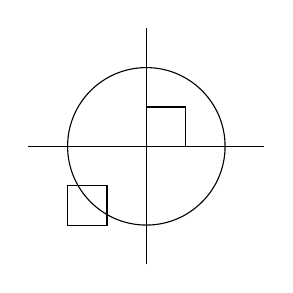
\begin{tikzpicture}
            \draw (-1.5,0) -- (1.5,0);
            \draw (0,-1.5) -- (0,1.5);
            \draw (0,0) circle [radius=1cm];
            \draw (0,0) rectangle (0.5,0.5);
            \draw (-0.5,-0.5) rectangle (-1,-1);
        \end{tikzpicture}
    \end{minipage}
    \begin{minipage}{0.55\linewidth}
        \begin{lstlisting}[style = latex-side]
    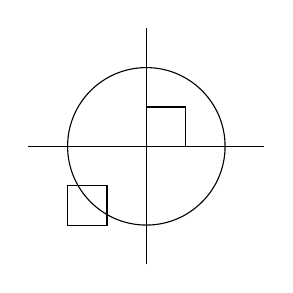
\begin{tikzpicture}
        \draw (-1.5,0) -- (1.5,0);
        \draw (0,-1.5) -- (0,1.5);
        \draw (0,0) circle [radius=1cm];
        \draw (0,0) rectangle (0.5,0.5);
        \draw (-0.5,-0.5) rectangle (-1,-1);
    \end{tikzpicture}
            \end{lstlisting}
    \end{minipage}
    \caption{带矩形的单位圆}
\end{figure}

\subsection{网格}
\subsubsection{网格的绘制}

网格的绘制形式:
\begin{lstlisting}[style = latex]
    \draw[step=2pt] (0,0) grid (10pt,10pt);
\end{lstlisting}
与曲线不同的是,第一个坐标点表示网格一个角,第二个坐标点则表示另一个不相邻的角,由此,我们可以在坐标轴基础上绘制网格背景了
\begin{figure}[H]
    \centering
    \begin{minipage}{0.35\linewidth}
        \centering
        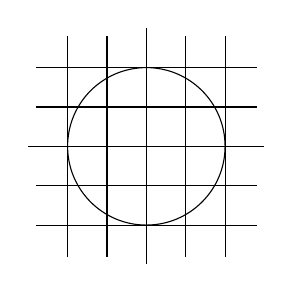
\begin{tikzpicture}
            \draw (-1.5,0) -- (1.5,0);
            \draw (0,-1.5) -- (0,1.5);
            \draw (0,0) circle [radius=1cm];
            \draw[step=.5cm] (-1.4,-1.4) grid (1.4,1.4);
            \end{tikzpicture}
    \end{minipage}
    \begin{minipage}{0.55\linewidth}
        \begin{lstlisting}[style = latex-side]
    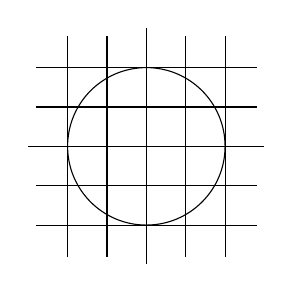
\begin{tikzpicture}
        \draw (-1.5,0) -- (1.5,0);
        \draw (0,-1.5) -- (0,1.5);
        \draw (0,0) circle [radius=1cm];
        \draw[step=.5cm] (-1.4,-1.4) grid (1.4,1.4);
        \end{tikzpicture}
            \end{lstlisting}
    \end{minipage}
    \caption{带网格的坐标轴}
\end{figure}

网格的颜色与单位圆相同,不易区别,这里使用更多的参数来控制

\begin{figure}[H]
    \centering
    \begin{minipage}{0.35\linewidth}
        \centering
        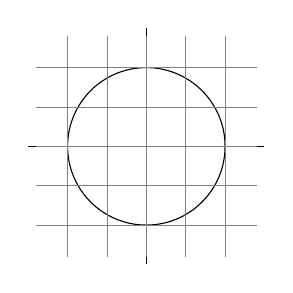
\begin{tikzpicture}
            \draw (-1.5,0) -- (1.5,0);
            \draw (0,-1.5) -- (0,1.5);
            \draw (0,0) circle [radius=1cm];
            \draw[step=.5cm,gray,very thin] (-1.4,-1.4) grid (1.4,1.4);
            \end{tikzpicture}
    \end{minipage}
    \begin{minipage}{0.55\linewidth}
        \begin{lstlisting}[style = latex-side]
    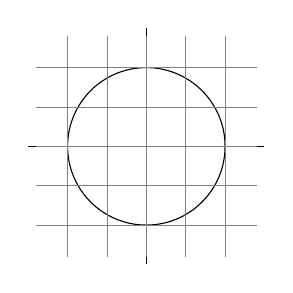
\begin{tikzpicture}
        \draw (-1.5,0) -- (1.5,0);
        \draw (0,-1.5) -- (0,1.5);
        \draw (0,0) circle [radius=1cm];
        \draw[step=.5cm,gray,very thin] (-1.4,-1.4) grid (1.4,1.4);
        \end{tikzpicture}
            \end{lstlisting}
    \end{minipage}
    \caption{修改颜色的带网格的坐标轴}
\end{figure}

\subsubsection{样式设置}
图像中的样式
对于进场重复使用的样式,我们可以设置一个统一样式,如网格虚线,我们定义为辅助线 help lines。

\begin{lstlisting}[style = latex]
   help lines/. style={color=blue!50,very thin}
\end{lstlisting}

全局样式
除了在图像中定义样式供单个图像使用,还可以定义全局样式。全局样式允许嵌套
\begin{lstlisting}[style = latex]
   \tikzset{help lines/.style=very thin}
   \tikzset{Pionpill gird/.style={help lines,color = blue!50}}
\end{lstlisting}

样式同时可以设置参数

\begin{figure}[H]
    \centering
    \begin{minipage}{0.35\linewidth}
        \centering
        \begin{tikzpicture}
            [Karl's grid/.style ={help lines,color=#1!50},
            Karl's grid/.default=blue]
            \draw[Karl's grid] (0,0) grid (1.5,2);
            \draw[Karl's grid=red] (2,0) grid (3.5,2);
       \end{tikzpicture}
    \end{minipage}
    \begin{minipage}{0.55\linewidth}
       \begin{lstlisting}[style = latex-side]
    \begin{tikzpicture}
        [Karl's grid/.style ={help lines,color=#1!50},
        Karl's grid/.default=blue]
        \draw[Karl's grid] (0,0) grid (1.5,2);
        \draw[Karl's grid=red] (2,0) grid (3.5,2);
        \end{tikzpicture}
       \end{lstlisting}
   \end{minipage}
   \caption{带参数的样式}
\end{figure}

网格除了以上重要参数,还有虚线参数可以设置 dash pattern

\subsection{弧度}
绘制弧度的形式:
\begin{lstlisting}[style = latex]
    \draw (x,y) arc [args]
\end{lstlisting}
和网格类使,第一个坐标表示弧线起点,arc 为关键词,之后为样式参数,默认为逆时针旋转

\begin{figure}[H]
    \centering
    \begin{minipage}{0.35\linewidth}
        \centering
        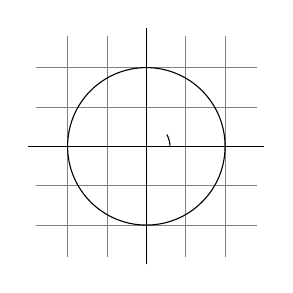
\begin{tikzpicture}
            \draw[step=.5cm,gray,very thin] (-1.4,-1.4) grid (1.4,1.4);
            \draw(-1.5,0) -- (1.5,0);
            \draw(0,-1.5) -- (0,1.5);
            \draw(0,0) circle [radius=1cm];
            \draw(3mm,0mm) arc [start angle=0,end angle=30,radius=3mm];
        \end{tikzpicture}
    \end{minipage}
    \begin{minipage}{0.55\linewidth}
        \begin{lstlisting}[style = latex-side]
    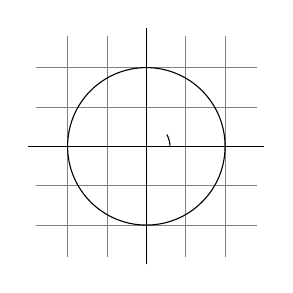
\begin{tikzpicture}
        \draw[step=.5cm,gray,very thin] (-1.4,-1.4) grid (1.4,1.4);
        \draw(-1.5,0) -- (1.5,0);
        \draw(0,-1.5) -- (0,1.5);
        \draw(0,0) circle [radius=1cm];
        \draw(3mm,0mm) arc [start angle=0,end angle=30,radius=3mm];
    \end{tikzpicture}
        \end{lstlisting}
    \end{minipage}
    \caption{带弧度的单位圆}
\end{figure}

如果对图像大小不满意,可以使用 tikzpicture 的 scale 参数进行放大

\begin{figure}[H]
    \centering
    \begin{minipage}{0.35\linewidth}
        \centering
        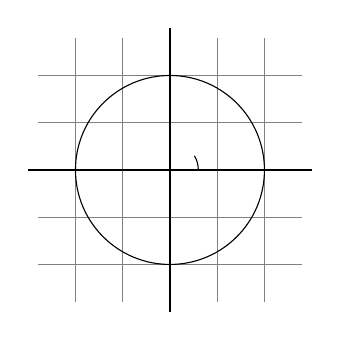
\begin{tikzpicture}[scale=1.2]
            \draw[step=.5cm,gray,very thin] (-1.4,-1.4) grid (1.4,1.4);
            \draw (-1.5,0) -- (1.5,0);
            \draw (0,-1.5) -- (0,1.5);
            \draw (0,0) circle [radius=1cm];
            \draw (3mm,0mm) arc [start angle=0, end angle=30, radius=3mm];
        \end{tikzpicture}
    \end{minipage}
    \begin{minipage}{0.55\linewidth}
        \centering
        \begin{lstlisting}[style = latex-side]
    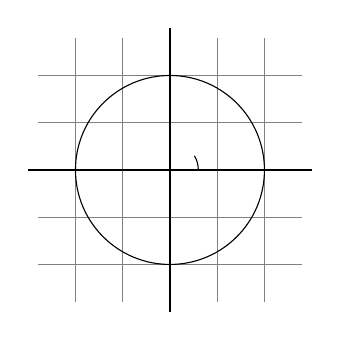
\begin{tikzpicture}[scale=1.2]
        \draw[step=.5cm,gray,very thin] (-1.4,-1.4) grid (1.4,1.4);
        \draw (-1.5,0) -- (1.5,0);
        \draw (0,-1.5) -- (0,1.5);
        \draw (0,0) circle [radius=1cm];
        \draw (3mm,0mm) arc [start angle=0, end angle=30, radius=3mm];
        \end{tikzpicture}
        \end{lstlisting}
    \end{minipage}
    \caption{放大后的图像}
\end{figure}

除了圆弧,还能绘制椭圆弧

\begin{figure}[H]
    \centering
    \begin{minipage}{0.35\linewidth}
        \centering
        \tikz \draw (0,0) arc [start angle=0, end angle=315, x radius=1.75cm, y radius=1cm];
    \end{minipage}
    \begin{minipage}{0.55\linewidth}
        \begin{lstlisting}[style = latex-side]
    \tikz \draw (0,0) arc [start angle=0, end angle=315, x radius=1.75cm, y radius=1cm];
        \end{lstlisting}
    \end{minipage}
    \caption{椭圆弧}
\end{figure}

\subsection{截图}
截图的用法与网格十分相识,可以指定截图方式,以及截图的对角来划定区域
\begin{lstlisting}[style = latex]
    \clip (x,y) graph (x,y)
\end{lstlisting}
需要注意的是,clip 指令需要写在前面的位置,下面使用矩形截图:
\begin{figure}[H]
    \centering
    \begin{minipage}{0.35\linewidth}
        \centering
        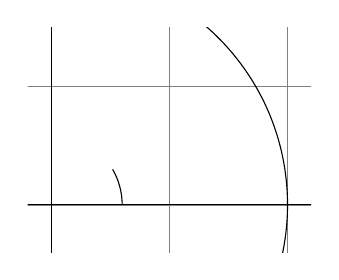
\begin{tikzpicture}[scale = 3]
            \clip (-0.1,-0.2) rectangle (1.1,0.75);
            \draw[step=.5cm,gray,very thin] (-1.4,-1.4) grid (1.4,1.4);
            \draw (-1.5,0) -- (1.5,0);
            \draw (0,-1.5) -- (0,1.5);
            \draw (0,0) circle [radius = 1cm];
            \draw (3mm,0mm) arc [start angle=0, end angle=30, radius=3mm];
        \end{tikzpicture}
    \end{minipage}
    \begin{minipage}{0.55\linewidth}
        \begin{lstlisting}[style = latex-side]
    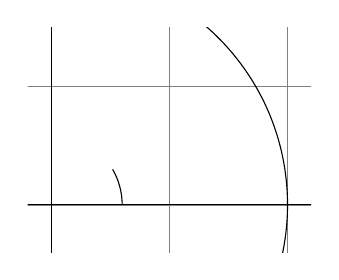
\begin{tikzpicture}[scale = 3]
        \clip (-0.1,-0.2) rectangle (1.1,0.75);
        \draw[step=.5cm,gray,very thin] (-1.4,-1.4) grid (1.4,1.4);
        \draw (-1.5,0) -- (1.5,0);
        \draw (0,-1.5) -- (0,1.5);
        \draw (0,0) circle [radius = 1cm];
        \draw (3mm,0mm) arc [start angle=0, end angle=30, radius=3mm];
    \end{tikzpicture}
        \end{lstlisting}
    \end{minipage}
    \caption{矩形截图}
\end{figure}

下面结合 draw 绘制圆形截图,技术细节不在此讨论

\begin{figure}[H]
    \centering
    \begin{minipage}{0.35\linewidth}
        \centering
        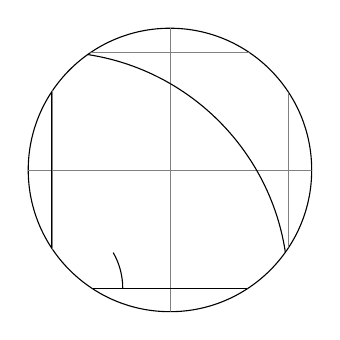
\begin{tikzpicture}[scale=3]
            \clip[draw] (0.5,0.5) circle (.6cm);
            \draw[step=.5cm,gray,very thin] (-1.4,-1.4) grid (1.4,1.4);
            \draw (-1.5,0) -- (1.5,0);
            \draw (0,-1.5) -- (0,1.5);
            \draw (0,0) circle [radius=1cm];
            \draw (3mm,0mm) arc [start angle=0, end angle=30, radius=3mm];
        \end{tikzpicture}
    \end{minipage}
    \begin{minipage}{0.55\linewidth}
        \begin{lstlisting}[style = latex-side]
    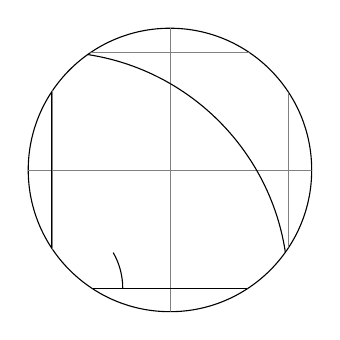
\begin{tikzpicture}[scale=3]
        \clip[draw] (0.5,0.5) circle (.6cm);
        \draw[step=.5cm,gray,very thin] (-1.4,-1.4) grid (1.4,1.4);
        \draw (-1.5,0) -- (1.5,0);
        \draw (0,-1.5) -- (0,1.5);
        \draw (0,0) circle [radius=1cm];
        \draw (3mm,0mm) arc [start angle=0, end angle=30, radius=3mm];
    \end{tikzpicture}
        \end{lstlisting}
    \end{minipage}
    \caption{结合 draw 绘制圆形截图}
\end{figure}

\subsection{抛物线与三角函数}
\subsubsection{抛物线}
抛物线同样使用 draw 命令绘制
\begin{figure}[H]
    \centering
    \begin{minipage}{0.35\linewidth}
        \centering
        \begin{tikzpicture}
            \draw (0,0) parabola (1,1);
        \end{tikzpicture}
    \end{minipage}
    \begin{minipage}{0.55\linewidth}
        \begin{lstlisting}[style = latex-side]
    \tikz \draw (0,0) parabola (1,1)
        \end{lstlisting}
    \end{minipage}
    \caption{抛物线}
\end{figure}

其他形式的抛物线
\begin{figure}[H]
    \centering
    \begin{minipage}{0.35\linewidth}
        \centering
        \begin{tikzpicture}
            \draw[x=1pt,y=1pt] (0,0) parabola bend (4,16) (6,12);
        \end{tikzpicture}
    \end{minipage}
    \begin{minipage}{0.55\linewidth}
        \begin{lstlisting}[style = latex-side]
    \tikz \draw[x=1pt,y=1pt] (0,0) parabola bend (4,16) (6,12)
        \end{lstlisting}
    \end{minipage}
    \caption{其他形式抛物线}
\end{figure}

\subsubsection{三角函数}
三角函数同样使用 draw 指令绘制
\begin{lstlisting}[style = latex]
    \draw[x=,y=] (x,y) sin (x,y)
\end{lstlisting}
其中,可选项 [x=,y=] 用于控制图像比例,第一个点为起点,随后指定三角函数类型,最后一个点为终点

\begin{figure}[H]
    \centering
    \begin{minipage}{0.35\linewidth}
        \centering
        \begin{tikzpicture}[scale = 1]
            \draw[x=1ex,y=1ex] (0,0) sin (1.57,1);
        \end{tikzpicture}
    \end{minipage}
    \begin{minipage}{0.55\linewidth}
        \begin{lstlisting}[style = latex-side]
            \tikz \draw[x=1ex,y=1ex] (0,0) sin (1.57,1);
        \end{lstlisting}
    \end{minipage}
    \caption{部分三角函数图像}
\end{figure}

\begin{figure}[H]
    \centering
    \begin{minipage}{0.35\linewidth}
        \centering
        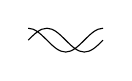
\begin{tikzpicture}[scale = 1]
            \draw [x=1.57ex,y=1ex] (0,0) sin(1,1) cos(2,0) sin(3,-1) cos(4,0) 
                                    (0,1) cos(1,0) sin(2,-1) cos(3,0) sin(4,1);
        \end{tikzpicture}
    \end{minipage}
    \begin{minipage}{0.55\linewidth}
        \begin{lstlisting}[style = latex-side]
    \tikz \draw [x=1.57ex,y=1ex] (0,0) sin(1,1) cos(2,0) sin(3,-1) cos(4,0) (0,1) cos(1,0) sin(2,-1) cos(3,0) sin(4,1);
        \end{lstlisting}
    \end{minipage}
    \caption{三角函数图像}
\end{figure}

\subsection{填充与边线}
\subsubsection{基本填充与边线}
使用 fill 代替 draw 关键字可绘制填充图形

\begin{figure}[H]
    \centering
    \begin{minipage}{0.35\linewidth}
        \centering
        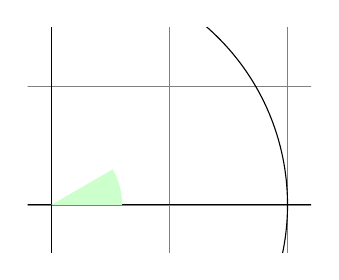
\begin{tikzpicture}[scale = 3]
            \clip (-0.1,-0.2) rectangle (1.1,0.75);
            \draw[step=.5cm,gray,very thin] (-1.4,-1.4) grid (1.4,1.4);
            \draw (-1.5,0) -- (1.5,0);
            \draw (0,-1.5) -- (0,1.5);
            \draw (0,0) circle [radius=1cm];
            \fill[green!20!white] (0,0) -- (3mm,0mm)
            arc [start angle=0, end angle=30, radius=3mm] -- (0,0);
        \end{tikzpicture}
    \end{minipage}
    \begin{minipage}{0.55\linewidth}
        \begin{lstlisting}[style = latex-side]
    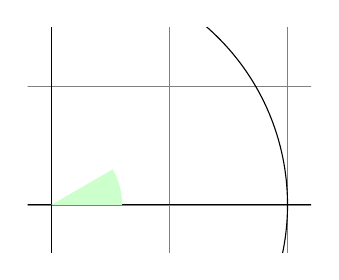
\begin{tikzpicture}[scale = 3]
        \clip (-0.1,-0.2) rectangle (1.1,0.75);
        \draw[step=.5cm,gray,very thin] (-1.4,-1.4) grid (1.4,1.4);
        \draw (-1.5,0) -- (1.5,0);
        \draw (0,-1.5) -- (0,1.5);
        \draw (0,0) circle [radius=1cm];
        \fill[green!20!white] (0,0) -- (3mm,0mm)
        arc [start angle=0, end angle=30, radius=3mm] -- (0,0);
    \end{tikzpicture}
        \end{lstlisting}
    \end{minipage}
    \caption{填充图形}
\end{figure}

边框线:useasboundingbox 
\begin{lstlisting}[style = latex]
    \useasboundingbox (low,high)
\end{lstlisting}
low 和 high 分别代表原边界向内,向外扩展,可使用 cycle 来指明曲线闭合

\begin{figure}[H]
    \centering
    \begin{minipage}{0.35\linewidth}
        \centering
        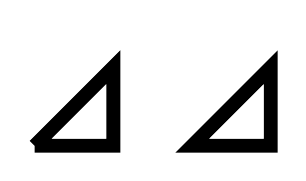
\begin{tikzpicture}[line width=5pt]
            \draw (0,0) -- (1,0) -- (1,1) -- (0,0);
            \draw (2,0) -- (3,0) -- (3,1) -- cycle;
            \useasboundingbox (0,1.5); % make bounding box higher
        \end{tikzpicture}
    \end{minipage}
    \begin{minipage}{0.55\linewidth}
        \begin{lstlisting}[style = latex-side]
    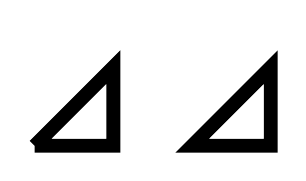
\begin{tikzpicture}[line width=5pt]
        \draw (0,0) -- (1,0) -- (1,1) -- (0,0);
        \draw (2,0) -- (3,0) -- (3,1) -- cycle;
        \useasboundingbox (0,1.5); % make bounding box higher
    \end{tikzpicture}
        \end{lstlisting}
    \end{minipage}
    \caption{边框粗细与闭合}
\end{figure}

可以使用 filldraw 绘制有边界线和填充的图形

\begin{figure}[H]
    \centering
    \begin{minipage}{0.35\linewidth}
        \centering
        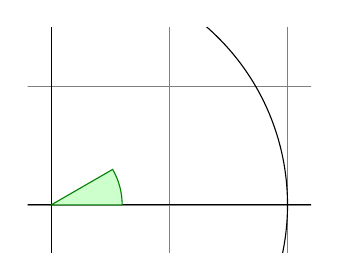
\begin{tikzpicture}[scale = 3]
            \clip (-0.1,-0.2) rectangle (1.1,0.75);
            \draw[step=.5cm,gray,very thin] (-1.4,-1.4) grid (1.4,1.4);
            \draw (-1.5,0) -- (1.5,0);
            \draw (0,-1.5) -- (0,1.5);
            \draw (0,0) circle [radius=1cm];
            \filldraw[fill=green!20!white, draw=green!50!black] (0,0) -- (3mm,0mm) arc [start angle=0, end angle=30, radius=3mm] -- cycle;
        \end{tikzpicture}
    \end{minipage}
    \begin{minipage}{0.55\linewidth}
        \begin{lstlisting}[style = latex-side]
    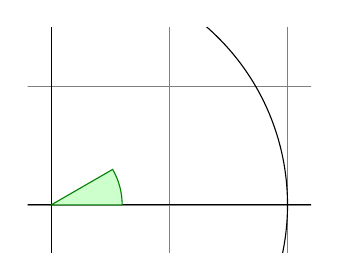
\begin{tikzpicture}[scale = 3]
        \clip (-0.1,-0.2) rectangle (1.1,0.75);
        \draw[step=.5cm,gray,very thin] (-1.4,-1.4) grid (1.4,1.4);
        \draw (-1.5,0) -- (1.5,0);
        \draw (0,-1.5) -- (0,1.5);
        \draw (0,0) circle [radius=1cm];
        \filldraw[fill=green!20!white, draw=green!50!black] (0,0) -- (3mm,0mm) arc [start angle=0, end angle=30, radius=3mm] -- cycle;
    \end{tikzpicture}
        \end{lstlisting}
    \end{minipage}
    \caption{filldraw 效果}
\end{figure}

\subsubsection{渐变}
与填充类使,渐变也有两种画法 shade 与 shadedraw

\begin{figure}[H]
    \centering
    \begin{minipage}{0.35\linewidth}
        \centering
        
\begin{tikzpicture}[scale = 1]
            \shade (0,0) rectangle (2,1) (3,0.5) circle (.5cm);
        \end{tikzpicture}
    \end{minipage}
    \begin{minipage}{0.55\linewidth}
        \begin{lstlisting}[style = latex-side]
    \tikz \shade (0,0) rectangle (2,1) (3,0.5) circle (.5cm)
        \end{lstlisting}
    \end{minipage}
    \caption{shade 效果}
\end{figure}

更详细的渐变设置

\begin{figure}[H]
    \centering
    \begin{minipage}{1\linewidth}
        \centering
        
\begin{tikzpicture}[scale = 1]
            \shade [top color=yellow,bottom color=black] (0,0) rectangle + (2,1);
            \shade[left color=yellow,right color=black] (3,0) rectangle +(2,1);
            \shadedraw[inner color=yellow,outer color=black,draw=yellow] (6,0) rectangle +(2,1);
            \shade[ball color=green] (9,.5) circle (.5cm);
        \end{tikzpicture}
    \end{minipage}
    \begin{minipage}{0.8\linewidth}
        \begin{lstlisting}[style = latex-side]
    
\begin{tikzpicture}[scale = 1]
        \shade [top color=yellow,bottom color=black] (0,0) rectangle + (2,1);
        \shade[left color=yellow,right color=black] (3,0) rectangle +(2,1);
        \shadedraw[inner color=yellow,outer color=black,draw=yellow] (6,0) rectangle +(2,1);
        \shade[ball color=green] (9,.5) circle (.5cm);
    \end{tikzpicture}
        \end{lstlisting}
    \end{minipage}
    \caption{几种渐变样式}
\end{figure}

尝试绘制新的圆弧
\begin{figure}[H]
    \centering
    \begin{minipage}{0.35\linewidth}
        \centering
        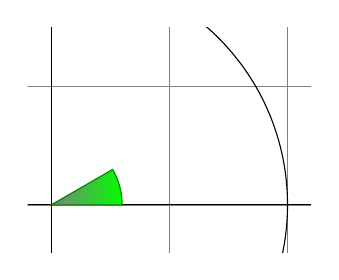
\begin{tikzpicture}[scale = 3]
            \clip (-0.1,-0.2) rectangle (1.1,0.75);
            \draw[step=.5cm,gray,very thin] (-1.4,-1.4) grid (1.4,1.4);
            \draw (-1.5,0) -- (1.5,0);
            \draw (0,-1.5) -- (0,1.5);
            \draw (0,0) circle [radius=1cm];
            \shadedraw[left color=gray,right color=green, draw=green!50!black] (0,0) -- (3mm,0mm)arc [start angle=0, end angle=30, radius=3mm] -- cycle;
        \end{tikzpicture}
    \end{minipage}
    \begin{minipage}{0.55\linewidth}
        \begin{lstlisting}[style = latex-side]
    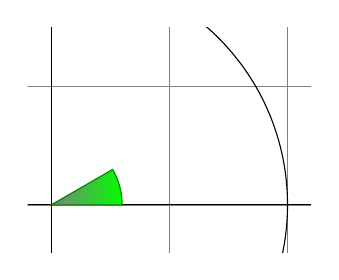
\begin{tikzpicture}[scale = 3]
        \clip (-0.1,-0.2) rectangle (1.1,0.75);
        \draw[step=.5cm,gray,very thin] (-1.4,-1.4) grid (1.4,1.4);
        \draw (-1.5,0) -- (1.5,0);
        \draw (0,-1.5) -- (0,1.5);
        \draw (0,0) circle [radius=1cm];
        \shadedraw[left color=gray,right color=green, draw=green!50!black] (0,0) -- (3mm,0mm)arc [start angle=0, end angle=30, radius=3mm] -- cycle;
    \end{tikzpicture}
        \end{lstlisting}
    \end{minipage}
    \caption{带渐变的圆弧}
\end{figure}

\subsection{指定坐标}
TikZ 指定坐标需要依靠数学计算,主要有两种方式
\begin{enumerate}
    \item 平面直角坐标系:例如:(10pt,2cm) 代表 x 方向偏移 10pt, y 方向偏移 2cm
    \item 极坐标系:例如:(30:1cm) 代表,逆时针选择 30$^{\circ}$, 长度为 1cm
\end{enumerate}

在确定坐标之后便可以依照新的点绘制图像,例如 +(0cm,1cm) 代表在坐标上方绘制 1cm 长线,++(2cm,0cm) 则再次绘制线段

\begin{figure}[H]
    \centering
    \begin{minipage}{0.35\linewidth}
        \centering
        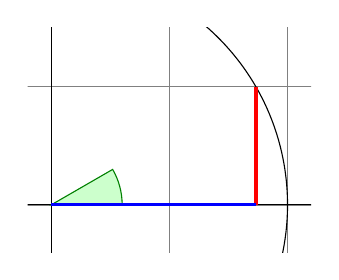
\begin{tikzpicture}[scale = 3]
            \clip (-0.1,-0.2) rectangle (1.1,0.75);
            \draw[step=.5cm,gray,very thin] (-1.4,-1.4) grid (1.4,1.4);
            \draw (-1.5,0) -- (1.5,0);
            \draw (0,-1.5) -- (0,1.5);
            \draw (0,0) circle [radius=1cm];
            \filldraw[fill=green!20,draw=green!50!black] (0,0) -- (3mm,0mm) arc [start angle=0, end angle=30, radius=3mm] -- cycle;
            \draw[red,very thick] (30:1cm) -- +(0,-0.5);
            \draw[blue,very thick] (30:1cm) ++(0,-0.5) -- (0,0);
        \end{tikzpicture}
    \end{minipage}
    \begin{minipage}{0.6\linewidth}
        \begin{lstlisting}[style = latex-side]
    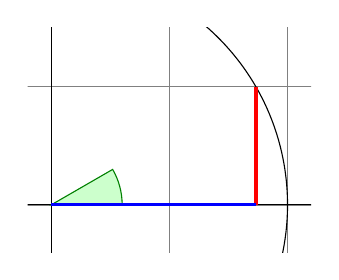
\begin{tikzpicture}[scale = 3]
        \clip (-0.1,-0.2) rectangle (1.1,0.75);
        \draw[step=.5cm,gray,very thin] (-1.4,-1.4) grid (1.4,1.4);
        \draw (-1.5,0) -- (1.5,0);
        \draw (0,-1.5) -- (0,1.5);
        \draw (0,0) circle [radius=1cm];
        \filldraw[fill=green!20,draw=green!50!black] (0,0) -- (3mm,0mm) arc [start angle=0, end angle=30, radius=3mm] -- cycle;
        \draw[red,very thick] (30:1cm) -- +(0,-0.5);
        \draw[blue,very thick] (30:1cm) ++(0,-0.5) -- (0,0);
    \end{tikzpicture}
        \end{lstlisting}
    \end{minipage}
    \caption{指定坐标绘制线段}
\end{figure}

从上述的例子可以发现,-- 承担了指定线段类型的责任,若没有 -- 则不会绘制线段,可以将这种用法用在定位点上,下面用几个例子详细说明 + 与 ++ 的作用

\begin{figure}[H]
    \centering
    \begin{minipage}{0.35\linewidth}
        \centering
        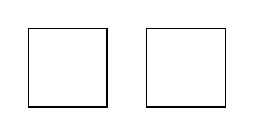
\begin{tikzpicture}[scale = 1]
            \def\rectanglepath{-- ++(1cm,0cm) -- ++(0cm,1cm) -- ++(-1cm,0cm) -- cycle}
            \draw (0,0) \rectanglepath;
            \draw (1.5,0) \rectanglepath;
        \end{tikzpicture}
    \end{minipage}
    \begin{minipage}{0.55\linewidth}
        \begin{lstlisting}[style = latex-side]
    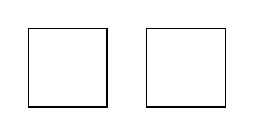
\begin{tikzpicture}[scale = 1]
        \def\rectanglepath{-- ++(1cm,0cm) -- ++(0cm,1cm) -- ++(-1cm,0cm) -- cycle}
        \draw (0,0) \rectanglepath;
        \draw (1.5,0) \rectanglepath;
    \end{tikzpicture}
        \end{lstlisting}
    \end{minipage}
    \caption{++ 绘制矩形}
\end{figure}

\begin{figure}[H]
    \centering
    \begin{minipage}{0.35\linewidth}
        \centering
        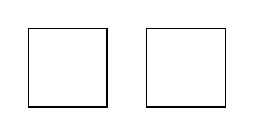
\begin{tikzpicture}[scale = 1]
            \def\rectanglepath{-- ++(1cm,0cm) -- ++(0cm,1cm) -- ++(-1cm,0cm) -- cycle}
            \draw (0,0) \rectanglepath;
            \draw (1.5,0) \rectanglepath;
        \end{tikzpicture}
    \end{minipage}
    \begin{minipage}{0.55\linewidth}
        \begin{lstlisting}[style = latex-side]
    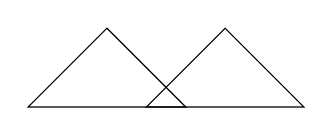
\begin{tikzpicture}[scale = 1]
        \def\rectanglepath{-- +(1cm,0cm) -- +(0cm,1cm) -- +(-1cm,0cm) -- cycle}
        \draw (0,0) \rectanglepath;
        \draw (1.5,0) \rectanglepath;
    \end{tikzpicture}
        \end{lstlisting}
    \end{minipage}
    \caption{+ 绘制矩形}
\end{figure}

\begin{figure}[H]
    \centering
    \begin{minipage}{0.35\linewidth}
        \centering
        \tikz \draw (0,0) rectangle +(1,1) (1.5,0) rectangle +(1,1);
    \end{minipage}
    \begin{minipage}{0.55\linewidth}
        \begin{lstlisting}[style = latex-side]
    \tikz \draw (0,0) rectangle +(1,1) (1.5,0) rectangle +(1,1);
        \end{lstlisting}
    \end{minipage}
    \caption{更快速的矩形绘制方式}
\end{figure}

\subsection{线段与箭头}
\subsubsection{箭头样式}
使用 -> 代替 -- 绘制有箭头的坐标轴

\begin{figure}[H]
    \centering
    \begin{minipage}{0.35\linewidth}
        \centering
        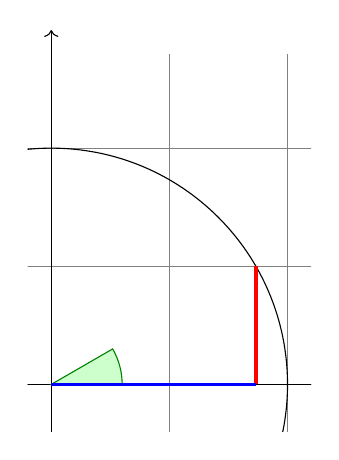
\begin{tikzpicture}[scale = 3]
            \clip (-0.1,-0.2) rectangle (1.1,1.51);
            \draw[step=.5cm,gray,very thin] (-1.4,-1.4) grid (1.4,1.4);
            \draw[->] (-1.5,0) -- (1.5,0);
            \draw[->] (0,-1.5) -- (0,1.5);
            \draw (0,0) circle [radius=1cm];
            \filldraw[fill=green!20,draw=green!50!black] (0,0) -- (3mm,0mm) arc [start angle=0, end angle=30, radius=3mm] -- cycle;
            \draw[red,very thick] (30:1cm) -- +(0,-0.5);
            \draw[blue,very thick] (30:1cm) ++(0,-0.5) -- (0,0);
        \end{tikzpicture}
    \end{minipage}
    \begin{minipage}{0.55\linewidth}
        \begin{lstlisting}[style = latex-side]
    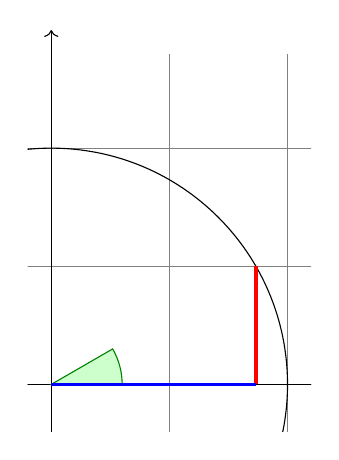
\begin{tikzpicture}[scale = 3]
        \clip (-0.1,-0.2) rectangle (1.1,1.51);
        \draw[step=.5cm,gray,very thin] (-1.4,-1.4) grid (1.4,1.4);
        \draw[->] (-1.5,0) -- (1.5,0);
        \draw[->] (0,-1.5) -- (0,1.5);
        \draw (0,0) circle [radius=1cm];
        \filldraw[fill=green!20,draw=green!50!black] (0,0) -- (3mm,0mm) arc [start angle=0, end angle=30, radius=3mm] -- cycle;
        \draw[red,very thick] (30:1cm) -- +(0,-0.5);
        \draw[blue,very thick] (30:1cm) ++(0,-0.5) -- (0,0);
    \end{tikzpicture}
        \end{lstlisting}
    \end{minipage}
    \caption{带箭头的坐标轴}
\end{figure}

可以在 draw 可选参数中使用箭头来指明箭头

\begin{figure}[H]
    \centering
    \begin{minipage}{0.35\linewidth}
        \centering
        \begin{tikzpicture}[scale = 1]
            \draw [<->] (0,0) arc [start angle = 180,end angle = 30, radius=10pt];
            \draw [<->] (1,0) -- (1.5cm,10pt) -- (2cm,0pt) -- (2.5cm,10pt);
        \end{tikzpicture}
    \end{minipage}
    \begin{minipage}{0.55\linewidth}
        \begin{lstlisting}[style = latex-side]
    \begin{tikzpicture}[scale = 1]
        \draw [<->] (0,0) arc [start angle = 180,end angle = 30, radius=10pt];
        \draw [<->] (1,0) -- (1.5cm,10pt) -- (2cm,0pt) -- (2.5cm,10pt);
    \end{tikzpicture}
        \end{lstlisting}
    \end{minipage}
    \caption{箭头示例}
\end{figure}

使用不一样的箭头样式
\begin{figure}[H]
    \centering
    \begin{minipage}{0.35\linewidth}
        \centering
        \usetikzlibrary {arrows.meta}
        \begin{tikzpicture}[scale = 1,>=Stealth]
            \draw [->] (0,0) arc [start angle=180, end angle=30,radius=10pt];
            \draw [<<-,very thick] (1,0) -- (1.5cm,10pt) -- (2cm,0pt) -- (2.5cm,10pt); 
        \end{tikzpicture}
    \end{minipage}
    \begin{minipage}{0.55\linewidth}
        \begin{lstlisting}[style = latex-side]
    \usetikzlibrary {arrows.meta}
    \begin{tikzpicture}[scale = 1,>=Stealth]
        \draw [->] (0,0) arc [start angle=180, end angle=30,radius=10pt];
        \draw [<<-,very thick] (1,0) -- (1.5cm,10pt) -- (2cm,0pt) -- (2.5cm,10py); 
    \end{tikzpicture}
        \end{lstlisting}
    \end{minipage}
    \caption{箭头样式}
\end{figure}

\subsubsection{范围 scope}
对于经常出现的同类样式,可以用 scope 设为统一样式

\begin{figure}[H]
    \centering
    \begin{minipage}{0.35\linewidth}
        \centering
        \begin{tikzpicture}[scale = 1,ultra thick]
            \draw (0,0) -- (0,1);
            \begin{scope}[thin]
                \draw (1,0) -- (1,1);
                \draw (2,0) -- (2,1);
            \end{scope}
            \draw (3,0) -- (3,1);
        \end{tikzpicture}
    \end{minipage}
    \begin{minipage}{0.55\linewidth}
        \begin{lstlisting}[style = latex-side]
    \begin{tikzpicture}[scale = 1,ultra thick]
        \draw (0,0) -- (0,1);
        \begin{scope}[thin]
            \draw (1,0) -- (1,1);
            \draw (2,0) -- (2,1);
        \end{scope}
        \draw (3,0) -- (3,1);
    \end{tikzpicture}
        \end{lstlisting}
    \end{minipage}
    \caption{scope 的作用}
\end{figure}

scope 还有一个重要作用,在 scope 内的操作只会影响内部范围

\subsection{位移}
可以使用 shift 关键字调整位置
\begin{figure}[H]
    \centering
    \begin{minipage}{0.35\linewidth}
        \centering
        \begin{tikzpicture}[scale = 1,rounded corners=2pt,x=15pt,y=15pt]
            \filldraw[fill=yellow!80!black] (0,0) rectangle (1,1)
                [xshift=5pt,yshift=5pt] (0,0) rectangle (1,1)
                    [rotate=30] (-1,-1) rectangle (2,2);
        \end{tikzpicture}
    \end{minipage}
    \begin{minipage}{0.56\linewidth}
        \begin{lstlisting}[style = latex-side]
    \begin{tikzpicture}[scale = 1,rounded corners=2pt,x=15pt,y=15pt]
        \filldraw[fill=yellow!80!black] (0,0) rectangle (1,1)
            [xshift=5pt,yshift=5pt] (0,0) rectangle (1,1)
                [rotate=30] (-1,-1) rectangle (2,2);
    \end{tikzpicture}
        \end{lstlisting}
    \end{minipage}
    \caption{位移示范}
\end{figure}

\subsection{循环}
\subsubsection{数字循环}

使用 foreach 指令,进行数字循环

\begin{lstlisting}[style = latex]
    \foreach <variable> in <values> <commands>
\end{lstlisting}

\begin{figure}[H]
    \centering
    \begin{minipage}{0.25\linewidth}
        \begin{tikzpicture}[scale = 1]
            \foreach \x in {1,2,3} {$x = \x$,}
        \end{tikzpicture}
    \end{minipage}
    \begin{minipage}{0.55\linewidth}
        \begin{lstlisting}[style = latex-side]
    \begin{tikzpicture}[scale = 1]
        \foreach \x in {1,2,3} {$x = \x$,}
    \end{tikzpicture}
        \end{lstlisting}
    \end{minipage}
    \caption{foreach 数字循环}
\end{figure}

同样,我们可以将其应用到绘图中

\begin{figure}[H]
    \centering
    \begin{minipage}{0.3\linewidth}
        \centering
        \begin{tikzpicture}[scale = 3]
            \clip (-0.1,-0.2) rectangle (1.1,1.51);
            \draw[step=.5cm,gray,very thin] (-1.4,-1.4) grid (1.4,1.4);
            \filldraw[fill=green!20,draw=green!50!black] (0,0) -- (3mm,0mm) arc [start angle=0, end angle=30, radius=3mm] -- cycle;
            \draw[->] (-1.5,0) -- (1.5,0);
            \draw[->] (0,-1.5) -- (0,1.5);
            \draw (0,0) circle [radius=1cm];
            \foreach \x in {-1cm,-0.5cm,1cm} \draw (\x,-1pt) -- (\x,1pt);
            \foreach \y in {-1cm,-0.5cm,0.5cm,1cm} \draw (-1pt,\y) -- (1pt,\y);
        \end{tikzpicture}
    \end{minipage}
    \begin{minipage}{0.65\linewidth}
        \begin{lstlisting}[style = latex-side]
    \begin{tikzpicture}[scale = 3]
        \clip (-0.1,-0.2) rectangle (1.1,1.51);
        \draw[step=.5cm,gray,very thin] (-1.4,-1.4) grid (1.4,1.4);
        \filldraw[fill=green!20,draw=green!50!black] (0,0) -- (3mm,0mm) arc [start angle=0, end angle=30, radius=3mm] -- cycle;
        \draw[->] (-1.5,0) -- (1.5,0);
        \draw[->] (0,-1.5) -- (0,1.5);
        \draw (0,0) circle [radius=1cm];
        \foreach \x in {-1cm,-0.5cm,1cm} \draw (\x,-1pt) -- (\x,1pt);
        \foreach \y in {-1cm,-0.5cm,0.5cm,1cm} \draw (-1pt,\y) -- (1pt,\y);
    \end{tikzpicture}
        \end{lstlisting}
    \end{minipage}
    \caption{循环绘制刻度线}
\end{figure}

再进一步,我们可以设计两个变量,绘制二维矩阵
\begin{figure}[H]
    \centering
    \begin{minipage}{1\linewidth}
        \centering
        \begin{tikzpicture}[scale = 1]
            \foreach \x in {1,2,...,5,7,8,...,12}
                \foreach \y in {1,...,5} {
                \draw (\x,\y) +(-.5,-.5) rectangle ++(.5,.5);
                \draw (\x,\y) node{\x,\y};
                }
        \end{tikzpicture}
    \end{minipage}
    \begin{minipage}{0.7\linewidth}
        \begin{lstlisting}[style = latex-side]
    \begin{tikzpicture}[scale = 1]
        \foreach \x in {1,2,...,5,7,8,...,12}
            \foreach \y in {1,...,5} {
            \draw (\x,\y) +(-.5,-.5) rectangle ++(.5,.5);
            \draw (\x,\y) node{\x,\y};
            }
    \end{tikzpicture}
        \end{lstlisting}
    \end{minipage}
    \caption{二维矩阵}
\end{figure}

\subsection{增加文字}
\subsubsection{node 关键字}
TikZ 可以通过 node 关键字指定节点并绘制区局,以达到添加文字的效果

\begin{figure}[H]
    \centering
    \begin{minipage}{0.35\linewidth}
        \centering
        \begin{tikzpicture}[scale = 1]
            \draw (0,0) rectangle (2,2);
            \draw (0.5,0.5) node [fill=gray!20] {Text 1} -- (1.5,1.5) node {Text2};
        \end{tikzpicture}
    \end{minipage}
    \begin{minipage}{0.55\linewidth}
        \begin{lstlisting}[style = latex-side]
    \begin{tikzpicture}[scale = 1]
        \draw (0,0) rectangle (2,2);
        \draw (0.5,0.5) node [fill=grey!20] {Text 1} -- (1.5,1.5) node {Text2}
    \end{tikzpicture}
        \end{lstlisting}
    \end{minipage}
    \caption{node 关键字的作用}
\end{figure}

默认将以 node 为几何中心构建方形区域,但也可自定义文字位置

\begin{figure}[H]
    \centering
    \begin{minipage}{0.35\linewidth}
        \centering
        \begin{tikzpicture}[scale = 3]
            \clip (-0.6,-0.2) rectangle (0.6,1.51);
            \draw[step=.5cm,help lines] (-1.4,-1.4) grid (1.4,1.4);
            \filldraw[fill=green!20,draw=green!50!black] (0,0) -- (3mm,0mm) arc [start angle=0, end angle=30, radius=3mm] -- cycle;
            \draw[->] (-1.5,0) -- (1.5,0); \draw[->] (0,-1.5) -- (0,1.5);
            \draw (0,0) circle [radius=1cm];
            \foreach \x in {-1,-0.5,1}
                \draw (\x cm,1pt) -- (\x cm,-1pt) node[anchor=north] {$\x$};
            \foreach \y in {-1,-0.5,0.5,1}
                \draw (1pt,\y cm) -- (-1pt,\y cm) node[anchor=east] {$\y$};
        \end{tikzpicture}
    \end{minipage}
    \begin{minipage}{0.6\linewidth}
        \begin{lstlisting}[style = latex-side]
    \begin{tikzpicture}[scale = 3]
        \clip (-0.6,-0.2) rectangle (0.6,1.51);
        \draw[step=.5cm,help lines] (-1.4,-1.4) grid (1.4,1.4);
        \filldraw[fill=green!20,draw=green!50!black] (0,0) -- (3mm,0mm) arc [start angle=0, end angle=30, radius=3mm] -- cycle;
        \draw[->] (-1.5,0) -- (1.5,0); \draw[->] (0,-1.5) -- (0,1.5);
        \draw (0,0) circle [radius=1cm];
        \foreach \x in {-1,-0.5,1}
            \draw (\x cm,1pt) -- (\x cm,-1pt) node[anchor=north] {$\x$};
        \foreach \y in {-1,-0.5,0.5,1}
            \draw (1pt,\y cm) -- (-1pt,\y cm) node[anchor=east] {$\y$};
    \end{tikzpicture}
        \end{lstlisting}
    \end{minipage}
    \caption{绘制坐标系制度}
\end{figure}

如果需要使用分数形式的文本,可以使用如下形式
\begin{lstlisting}[style = latex]
    \x / \xtex
\end{lstlisting}

\begin{figure}[H]
    \centering
    \begin{minipage}{0.3\linewidth}
        \centering
        \begin{tikzpicture}[scale = 3]
            \clip (-0.6,-0.2) rectangle (0.6,1.51);
            \draw[step=.5cm,help lines] (-1.4,-1.4) grid (1.4,1.4);
            \filldraw[fill=green!20,draw=green!50!black] (0,0) -- (3mm,0mm) arc [start angle=0, end angle=30, radius=3mm] -- cycle;
            \draw[->] (-1.5,0) -- (1.5,0); \draw[->] (0,-1.5) -- (0,1.5);
            \draw (0,0) circle [radius=1cm];
            \foreach \x/\xtext in {-1, -0.5/-\frac{1}{2}, 1}
                \draw (\x cm,1pt) -- (\x cm,-1pt) node[anchor=north] {$\xtext$};
            \foreach \y/\ytext in {-1, -0.5/-\frac{1}{2}, 0.5/\frac{1}{2}, 1}
                \draw (1pt,\y cm) -- (-1pt,\y cm) node[anchor=east] {$\ytext$};
        \end{tikzpicture}
    \end{minipage}
    \begin{minipage}{0.65\linewidth}
        \begin{lstlisting}[style = latex-side]
    \begin{tikzpicture}[scale = 3]
        \clip (-0.6,-0.2) rectangle (0.6,1.51);
        \draw[step=.5cm,help lines] (-1.4,-1.4) grid (1.4,1.4);
        \filldraw[fill=green!20,draw=green!50!black] (0,0) -- (3mm,0mm) arc [start angle=0, end angle=30, radius=3mm] -- cycle;
        \draw[->] (-1.5,0) -- (1.5,0); \draw[->] (0,-1.5) -- (0,1.5);
        \draw (0,0) circle [radius=1cm];
        \foreach \x/\xtext in {-1, -0.5/-\frac{1}{2}, 1}
            \draw (\x cm,1pt) -- (\x cm,-1pt) node[anchor=north] {$\xtext$};
        \foreach \y/\ytext in {-1, -0.5/-\frac{1}{2}, 0.5/\frac{1}{2}, 1}
            \draw (1pt,\y cm) -- (-1pt,\y cm) node[anchor=east] {$\ytext$};
    \end{tikzpicture}
        \end{lstlisting}
    \end{minipage}
    \caption{绘制坐标系制度(分数形式)}
\end{figure}

接着之前的直角坐标系,我们可以标出函数 (以下为官方代码,出现了部分前面未说明的内容)

\begin{figure}[H]
    \centering
    \begin{minipage}{1\linewidth}
        \centering
        \usetikzlibrary {intersections}
        \begin{tikzpicture}[scale=3.5]
            \clip (-2,-0.22) rectangle (2,0.8);
            \draw[step=.5cm,gray,very thin] (-1.4,-1.4) grid (1.4,1.4);
            \filldraw[fill=green!20,draw=green!50!black] (0,0) -- (3mm,0mm) arc [start angle=0, end angle=30, radius=3mm] -- cycle;
            \draw[->] (-1.5,0) -- (1.5,0) coordinate (x axis);
            \draw[->] (0,-1.5) -- (0,1.5) coordinate (y axis);
            \draw (0,0) circle [radius=1cm];
            \draw[very thick,red] (30:1cm) -- node[left=1pt,fill=white] {$\sin \alpha$} (30:1cm |- x axis);
            \draw[very thick,blue] (30:1cm |- x axis) -- node[below=2pt,fill=white] {$\cos \alpha$} (0,0);
            \path [name path=upward line] (1,0) -- (1,1);
            \path [name path=sloped line] (0,0) -- (30:1.5cm);
            \draw [name intersections={of=upward line and sloped line, by=t}] [very thick,orange] (1,0) -- node [right=1pt,fill=white] {$\displaystyle \tan \alpha \color{black}= \frac{{\color{red}\sin \alpha}}{\color{blue}\cos \alpha}$} (t);
            \draw (0,0) -- (t);
            \foreach \x/\xtext in {-1, -0.5/-\frac{1}{2}, 1}
                \draw (\x cm,1pt) -- (\x cm,-1pt) node[anchor=north,fill=white] {$\xtext$};
            \foreach \y/\ytext in {-1, -0.5/-\frac{1}{2}, 0.5/\frac{1}{2}, 1}
                \draw (1pt,\y cm) -- (-1pt,\y cm) node[anchor=east,fill=white] {$\ytext$};
        \end{tikzpicture}
    \end{minipage}
    \begin{minipage}{0.9\linewidth}
        \begin{lstlisting}[style = latex-side]
    \begin{tikzpicture}[scale=3.5]
        \clip (-2,-0.22) rectangle (2,0.8);
        \draw[step=.5cm,gray,very thin] (-1.4,-1.4) grid (1.4,1.4);
        \filldraw[fill=green!20,draw=green!50!black] (0,0) -- (3mm,0mm) arc [start angle=0, end angle=30, radius=3mm] -- cycle;
        \draw[->] (-1.5,0) -- (1.5,0) coordinate (x axis);
        \draw[->] (0,-1.5) -- (0,1.5) coordinate (y axis);
        \draw (0,0) circle [radius=1cm];
        \draw[very thick,red] (30:1cm) -- node[left=1pt,fill=white] {$\sin \alpha$} (30:1cm |- x axis);
        \draw[very thick,blue] (30:1cm |- x axis) -- node[below=2pt,fill=white] {$\cos \alpha$} (0,0);
        \path [name path=upward line] (1,0) -- (1,1);
        \path [name path=sloped line] (0,0) -- (30:1.5cm);
        \draw [name intersections={of=upward line and sloped line, by=t}] [very thick,orange] (1,0) -- node [right=1pt,fill=white] {$\displaystyle \tan \alpha \color{black}= \frac{{\color{red}\sin \alpha}}{\color{blue}\cos \alpha}$} (t);
        \draw (0,0) -- (t);
        \foreach \x/\xtext in {-1, -0.5/-\frac{1}{2}, 1}
            \draw (\x cm,1pt) -- (\x cm,-1pt) node[anchor=north,fill=white] {$\xtext$};
        \foreach \y/\ytext in {-1, -0.5/-\frac{1}{2}, 0.5/\frac{1}{2}, 1}
            \draw (1pt,\y cm) -- (-1pt,\y cm) node[anchor=east,fill=white] {$\ytext$};
    \end{tikzpicture}
        \end{lstlisting}
    \end{minipage}
    \caption{带文字的单位圆}
\end{figure}

\subsubsection{线段文字}
可以通过 sloped 关键字指定在线段的某一区域添加文字

\begin{figure}[H]
    \centering
    \begin{minipage}{1\linewidth}
        \centering
        \begin{tikzpicture}[scale = 1]
            \draw (0,0) .. controls (6,1) and (9,1) ..
                node [near start,sloped,above] {near start}
                node {midway}
                node [very near end,sloped,below] {very near end}(12,0);
        \end{tikzpicture}
    \end{minipage}
    \begin{minipage}{0.6\linewidth}
        \begin{lstlisting}[style = latex-side]
    \begin{tikzpicture}[scale = 1]
        \draw (0,0) .. controls (6,1) and (9,1) ..
            node [near start,sloped,above] {near start}
            node {midway}
            node [very near end,sloped,below] {very near end}(12,0);
    \end{tikzpicture}
        \end{lstlisting}
    \end{minipage}
    \caption{sloped 控制段落文字位置}
\end{figure}

\subsection{最终结果}
\begin{figure}[H]
    \centering
    \begin{minipage}{1\linewidth}
        \centering
        \begin{tikzpicture}
            [scale=3,line cap=round,
            % Styles
            axes/.style=,
            important line/.style={very thick},
            information text/.style={rounded corners,fill=red!10,inner sep=1ex}]

            % Colors
            \colorlet{anglecolor}{green!50!black}
            \colorlet{sincolor}{red}
            \colorlet{tancolor}{orange!80!black}
            \colorlet{coscolor}{blue}

            % The graphic
            \draw[help lines,step=0.5cm] (-1.4,-1.4) grid (1.4,1.4);

            \draw (0,0) circle [radius=1cm];

            \begin{scope}[axes]
                \draw[->] (-1.5,0) -- (1.5,0) node[right] {$x$} coordinate(x axis);
                \draw[->] (0,-1.5) -- (0,1.5) node[above] {$y$} coordinate(y axis);
                \foreach \x/\xtext in {-1, -.5/-\frac{1}{2}, 1}
                    \draw[xshift=\x cm] (0pt,1pt) -- (0pt,-1pt) node[below,fill=white] {$\xtext$};
                \foreach \y/\ytext in {-1, -.5/-\frac{1}{2}, .5/\frac{1}{2}, 1}
                    \draw[yshift=\y cm] (1pt,0pt) -- (-1pt,0pt) node[left,fill=white] {$\ytext$};
            \end{scope}
            
            \filldraw[fill=green!20,draw=anglecolor] (0,0) -- (3mm,0pt) arc [start angle=0, end angle=30, radius=3mm];
            \draw (15:2mm) node[anglecolor] {$\alpha$};
            \draw[important line,sincolor] (30:1cm) -- node[left=1pt,fill=white] {$\sin \alpha$} (30:1cm |- x axis);
            \draw[important line,coscolor] (30:1cm |- x axis) -- node[below=2pt,fill=white] {$\cos \alpha$} (0,0);
            \path [name path=upward line] (1,0) -- (1,1);
            \path [name path=sloped line] (0,0) -- (30:1.5cm);
            \draw [name intersections={of=upward line and sloped line, by=t}][very thick,orange] (1,0) -- node [right=1pt,fill=white]{$\displaystyle \tan \alpha \color{black}=\frac{{\color{red}\sin \alpha}}{\color{blue}\cos \alpha}$} (t);

            \draw (0,0) -- (t);

            \draw[xshift=1.85cm]
                node[right,text width=6cm,information text]{
                The {\color{anglecolor} angle $\alpha$} is $30^\circ$ in the example ($\pi/6$ in radians). The {\color{sincolor}sine of $\alpha$}, which is the height of the red line, is\[{\color{sincolor} \sin \alpha} = 1/2.\]By the Theorem of Pythagoras ...
                };
        \end{tikzpicture}
    \end{minipage}
    \caption{}
\end{figure}


\subsection{其他技巧}
可以使用 coordinate 指定点位置并赋予别名,并通过 pic 来进行快速绘图,pic 这里只做演示,详细内容后续章节会讲解

\begin{figure}[H]
    \centering
    \begin{minipage}{0.35\linewidth}
        \centering
        \usetikzlibrary {angles,quotes}
        \begin{tikzpicture}[scale = 3]
            \coordinate (A) at (1,0);
            \coordinate (B) at (0,0);
            \coordinate (C) at (30:1cm);
            \draw (A) -- (B) -- (C) pic [draw=green!50!black, fill=green!20, angle radius=9mm,"$\alpha$"] {angle = A--B--C};
        \end{tikzpicture}
    \end{minipage}
    \begin{minipage}{0.6\linewidth}
        \begin{lstlisting}[style = latex-side]
    \usetikzlibrary {angles,quotes}
    \begin{tikzpicture}[scale = 3]
        \coordinate (A) at (1,0);
        \coordinate (B) at (0,0);
        \coordinate (C) at (30:1cm);
        \draw (A) -- (B) -- (C)
            pic [draw=green!50!black, fill=green!20, angle radius=9mm,
                "$\alpha$"] {angle = A--B--C};
    \end{tikzpicture}
        \end{lstlisting}
    \end{minipage}
    \caption{使用 pic 快速绘制}
\end{figure}